\section{Jordfugt} \label{sec:JrdImpl}

Dette afsnit beskriver implementering af SW og HW i blokken Jordfugt. Afsnittet beskriver hhv. HW og SW i underblokken PSoC4.

\subsection{HW PSoC4}
\begin{figure}[h]
\centering 
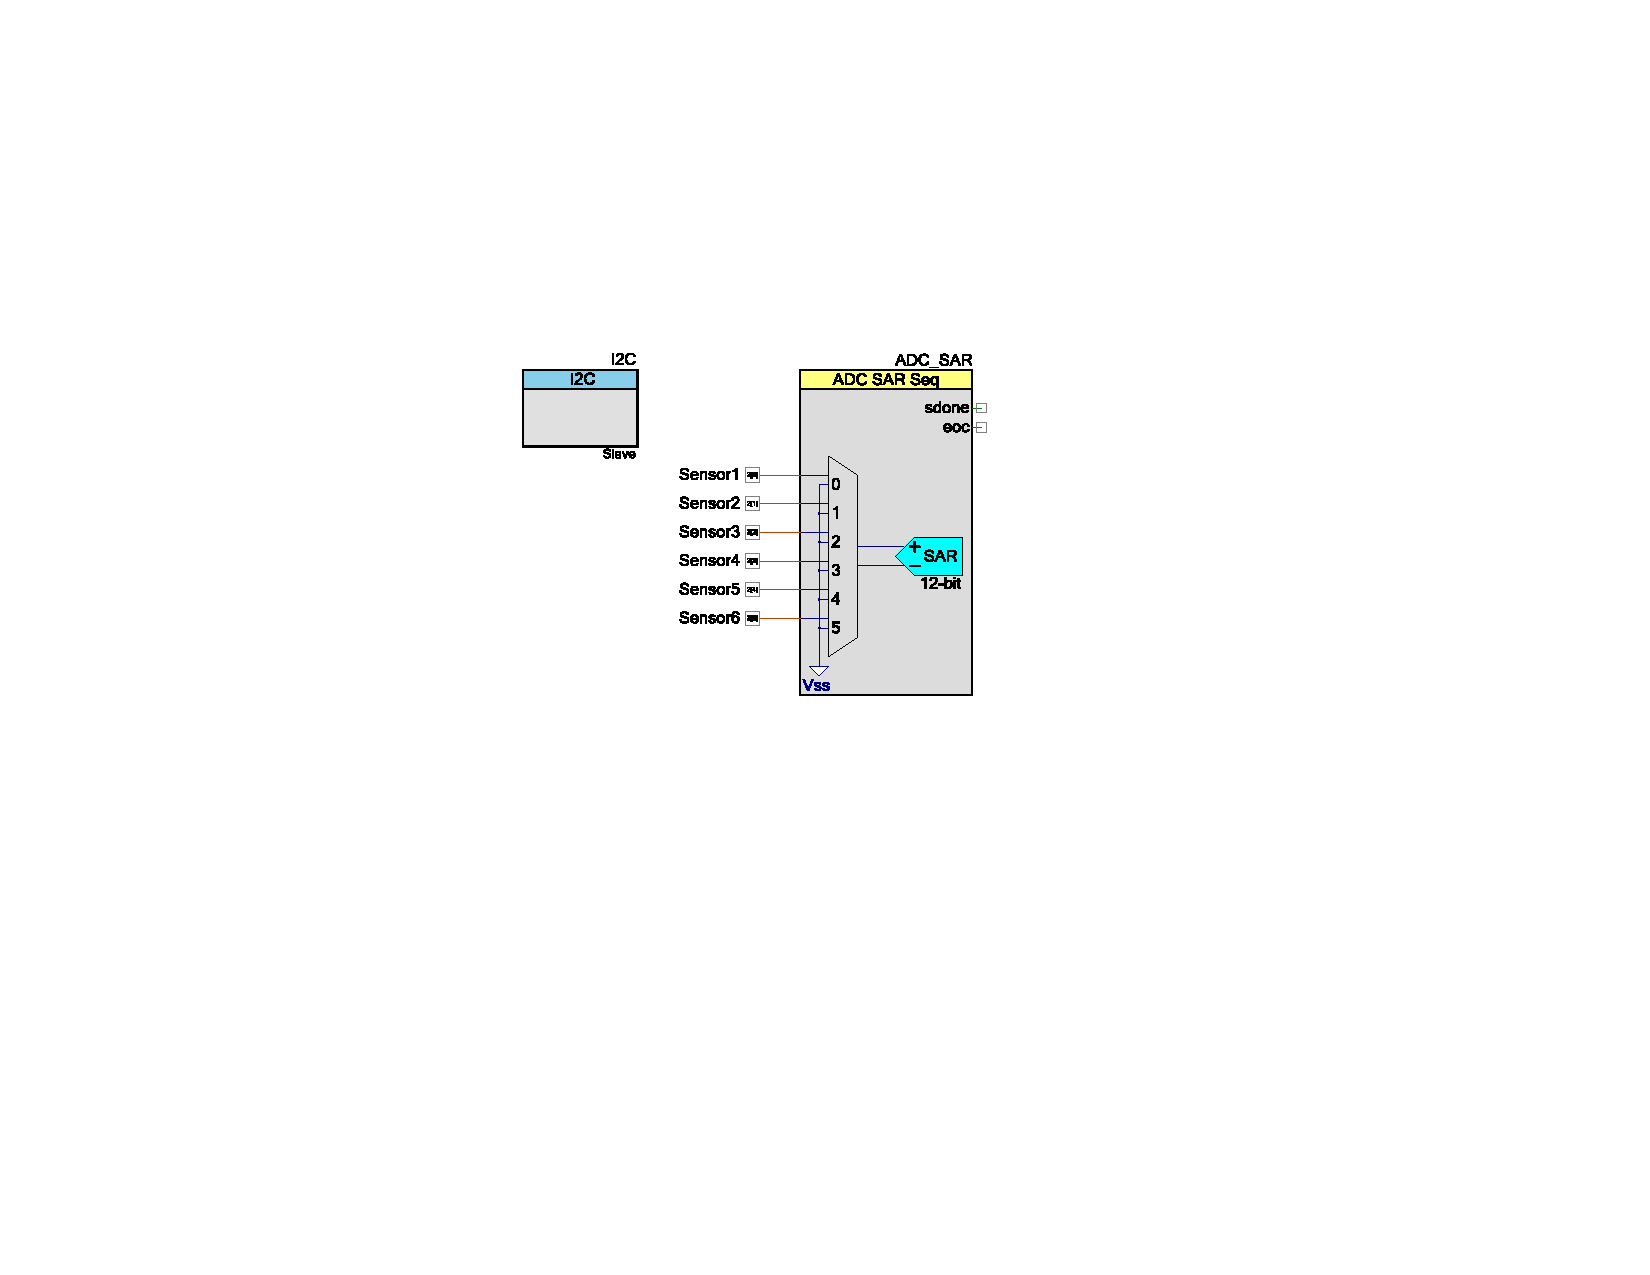
\includegraphics[width={\textwidth-6cm}, trim = 250 270 310 160, clip=true] {../fig/TopDesign_Jordfugt.pdf}
\caption{TopDesign.cysch for PSoC4 i Jordfugt}
\label{fig:topdesign_jordfugt}
\end{figure}

Den HW, der syntetiseres i PSoC4 Jordfugt er vist på figur\ref{fig:topdesign_jordfugt}. 

I2C komponenten styrer kommunikation med MasterPSoC via \IIC. 
Den konfigureret til at være slave med adressen 0x32, datarate er indstillet til 100 kbps.

ADC\_SAR komponenten er en Analog to Digital converter, med seks forskellige inputs. Referencespænding er konfigureret til VDDA (3.3V).
Indstillet til 8 bit præcision og en sample frekvens på 1 MHz, hvilket resulterer i en samplerate på 11904 SPS.

Alle pins i topdeignet er konfigureret til resistive pull down. 
Det vil sige at de altd er defineret low hvis der ikke er et sensor input.

\clearpage

\subsection{SW PSoC4}

\begin{lstlisting}[caption=Udsnit A af main.c for PSoC4 i Jordfugt, label=fig:main1_jordfugt]
int main()
{
    //Enable interrupts
    CyGlobalIntEnable; 
    
    //Initialisering af read og write buffere og start af I2C Slave.
    I2C_I2CSlaveInitReadBuf(readBuffer, RD_BUFFERSIZE);
    I2C_I2CSlaveInitWriteBuf(writeBuffer, WR_BUFFERSIZE);
    I2C_Start();
    
    //Start af ADC
    ADC_SAR_Start();
    ADC_SAR_StartConvert();

    for(;;)
    {
        checkForData();
        if(i < 6)
        {
            data = ADC_SAR_GetResult16(i); //Hent de oenskede data
            if ((data & 0b10000000) || (data > MAXIMUM) || (data < MINIMUM)) //Tjek om oenskede data er inden for graenser
            {
                convertedData = 0b10000000; //Skriv fejl til konvertede data
            }
            else
            {
                convertedData = (100 - (((data - MINIMUM)*100)/(MAXIMUM-MINIMUM))); //Konverter data til tal med vaerdi 0 - 100
            }
            readBuffer[0] = convertedData; //Goer data klar til aflaesning
            I2C_I2CSlaveClearReadBuf(); //Reset read buffer pointer
            i = 0xFFFFFFFF;
        }
    }
}

...
\end{lstlisting}

Svissen Svassen

\clearpage

\begin{lstlisting}[caption=Udsnit B af main.c for PSoC4 i Jordfugt, label=fig:main2_jordfugt]
...

void checkForData()
{
    //Check for om der er modtaget data
    if(I2C_I2CSlaveStatus() & I2C_I2C_SSTAT_WR_CMPLT)
    {
        //Put data i varibel i            
        i = writeBuffer[0] & 0b00000111;
        
        I2C_I2CSlaveClearWriteBuf(); //Clear buffer pointer
        I2C_I2CSlaveClearWriteStatus(); //Clear status                               
    }
}
\end{lstlisting}

Svissen Svassen

\clearpage